% $Date$
\documentclass[12pt,a4paper]{article}
\usepackage[polish]{babel}                      % Język polski
\usepackage[utf8]{inputenc}                     % Kodowanie dokumentu
\usepackage[T1]{fontenc}                        % Kodowanie fontów
%\usepackage{lmodern}
\usepackage{times}                              % Font wektorowy
\usepackage[cm]{fullpage}                       % Cała szerokość strony
\usepackage[pdftex,bookmarks,colorlinks]{hyperref} % Linki w dokumencie PDF
\usepackage{indentfirst}                        % Wcięcia akapitów
\usepackage{graphicx}                           % Grafika w png, jpeg, gif
%\pagestyle{headings}
%\graphicspath{{png}}                            % Szuka grafik w katalogu png
\frenchspacing                                  % Odstępy międzyzdaniowe

\title{ConvML 1.2}
\author{Marcin Kacprzak\\ marcin.kacprzak@entertech.com.pl\\
  \and Piotr Kulinowski\\ piotr.kulinowski@entertech.com.pl}
\date{\today}

\begin{document}

\maketitle

\begin{abstract}
  Ten dokument zawiera opis funkcji i składni języka ConvML.  ConvML jest językiem
  do zapisu strukturalnego modelu przenośnika taśmowego w formacie XML [XML10].

  Wersję PDF tego dokumentu można odnaleźć pod adresem
  \href{http://www.entertech.com.pl/convml/convml.pdf}{entertech.com.pl/convml/convml.pdf}.
\end{abstract}

\tableofcontents


\section{Wstęp}
Potrzeba opracowania modelu strukturalnego przenośnika taśmowego wynikła z
informatycznej konieczności wprowadzenia procedury zapisu pełnej informacji o
urządzeniu, która jednoznacznie i spójnie opisywałaby parametry
techniczno-ruchowe i konfigurację przenośnika taśmowego.  Ze względu na
uniwersalność zapisu i chęć popularyzacji modelu strukturalnego wprowadzono
anglojęzyczne nazewnictwo poszczególnych podzespołów.

Do opracowania systemu zapisu modelu strukturalnego przenośnika taśmowego
wykorzystano język XML Schema [XSD10], ułatwiający definiowanie struktury i
kolejności podzespołów przenośnika taśmowego (Tabela 4 1) oraz umożliwiający w
łatwy sposób jego adaptację na platformie informatycznej.  Istotną cechą modelu
strukturalnego jest praktycznie nieograniczona możliwość jego rozbudowy, bez
utraty przejrzystości struktury.  Każdy z elementów posiada grupę atrybutów
opisujących jego cechy, mogące być zarówno parametrami technicznymi jak i
ekonomicznymi.


\section{Konwencje}
Nazwa ConvML pochodzi od Conveyor Meta Language.  Typowy dokument ConvML ma
postać pliku tekstowego o rozszerzeniu xml lub convml.  Zalecane kodowanie to
UTF-8.

Dokument ConvML do zapisu informacji o strykturze przenośnika wykorzystuje
\emph{elementy}, a do zapisu właściwości używane są \emph{atrybuty} języka XML.
Elementy w języku ConvML mogą zawierać inne elementy oraz atrybuty, nie używa
się natomiast tekstu zawartego pomiędzy znacznikami do zapisu informacji o
przenośniku taśmowym.

Elementy języka ConvML należą do przestrzeni nazw:
http://www.entertech.com.pl/bcml.


\section{Struktura dokumentu}
Głównym elementem dokumentu jest ConvML.  Podelementy Meta oraz Types są
opcjonalne. Element BeltConveyor musi wystąpić co najmniej raz aby dokument był
poprawny.  Przykładowa instancja dokumentu może mieć następującą postać:

\begin{verbatim}
<?xml version="1.0" encoding="utf-8"?>
<ConvML version="1.2">
  <Meta/>
  <Types/>
  <BeltConveyor/>
</ConvML>
\end{verbatim}  


\subsection{Element główny <ConvML>}

\begin{figure}[h]
  \centering
  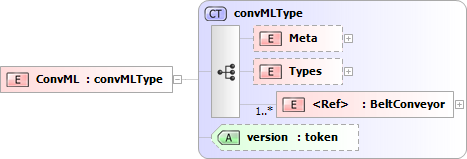
\includegraphics[width=0.6\textwidth]{png/convml_xsd2}
  \caption{Definicja elementu ConvML}
  \label{fig:convml-xsd}
\end{figure}

\paragraph{Definicje atrybutów:}
\begin{description}
\item[version] Zastosowana w dokumencie wersja języka ConvML.
\end{description}


\subsection{Przenośnik taśmowy <BeltConveyor>}
Górnicze przenośniki taśmowe definiuje się jako urządzenia służące do ciągłego
transportu na taśmie materiałów sypkich, pozyskiwanych podczas procesów
związanych z prowadzeniem robót górniczych [Kulinowski2011].  Do zespołów
głównych przenośnika taśmowego należą: stacja czołowa, stacja zwrotna, stacja
napinania taśmy, taśma, trasa, zestawy krążnikowe i krążniki [Antoniak2005].

\begin{figure}
  \centering
  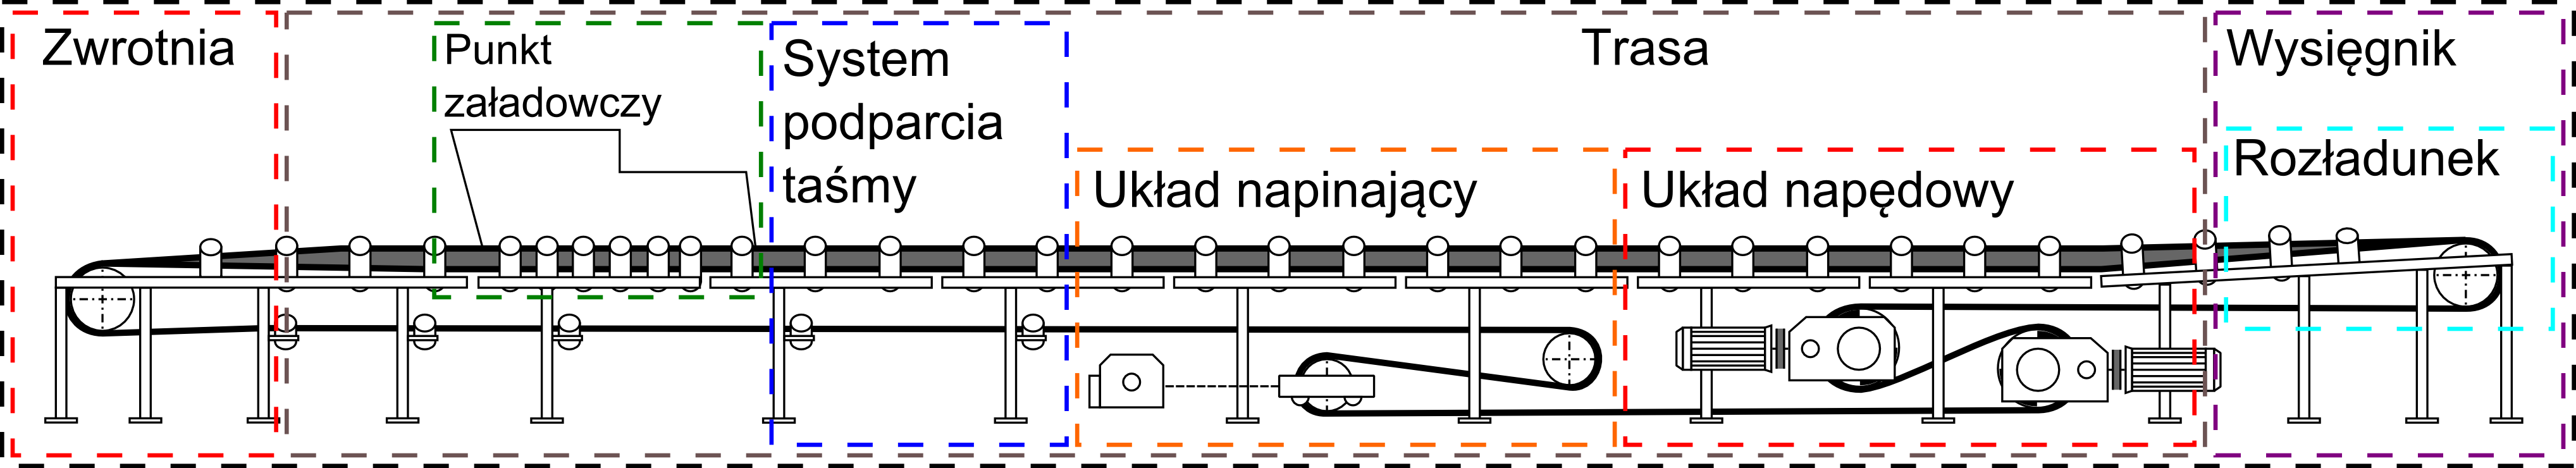
\includegraphics[width=\textwidth]{png/belt_conveyor_drw}
  \caption{Podstawowe podzespoły przenośnika taśmowego}
  \label{fig:beltConveyor-drw}
\end{figure}

W języku ConvML podstawowy podział przenośnika taśmowego wygląda następująco:

\begin{itemize}
\item Belt -- taśma,
\item Tail -- stacja zwrotna,
\item Route -- trasa,
\item Head -- stacja czołowa.
\end{itemize}

Pozostałe zespoły główne przenośnika taśmowego znajdują się głębiej w strukturze
opisywanej przez język ConvML.  System podparcia taśmy należy do elementów
składowych trasy.  Układy napędowy i napinający są powiązane z bębnami, które
mogą występować jako elementy składowe stacji zwrotnej, stacji czołowej lub
trasy.

\begin{figure}[h]
  \centering
  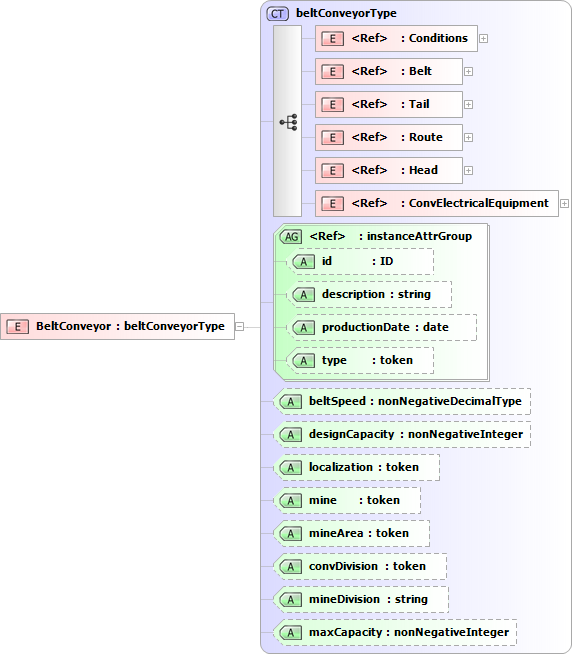
\includegraphics[width=0.6\textwidth]{png/belt_conveyor_xsd2}
  \caption{Definicja elementu BeltConveyor}
  \label{fig:beltConveyor-xsd}
\end{figure}

\paragraph{Definicje atrybutów:}
\begin{description}
\item[beltSpeed] Prędkość taśmy przenośnika - v [m/s].
\item[designCapacity] Wydajność nominalna przenośnika - Q [t/h].
\item[localization] Wyrobisko.
\item[mine] Kopalnia.
\item[mineArea] Rejon.
\item[convDivision] Oddział taśmowy.
\item[mineDivision] Obsługiwane oddziały wydobywcze.
\item[maxCapacity] Wydajność maksymalna.
\end{description}


\subsection{Warunki pracy przenośnika <Conditions>}
Element Conditions grupuje atrybuty związane z warunkami pracy przenośnika
taśmowego.

\begin{figure}[h]
  \centering
  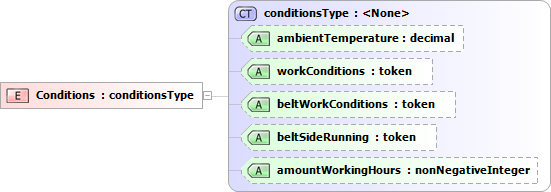
\includegraphics[width=0.6\textwidth]{png/conditions_xsd2}
  \caption{Definicja elementu Conditions}
  \label{fig:conditions-xsd}
\end{figure}

\paragraph{Definicje atrybutów:}
\begin{description}
\item[ambientTemperature] Temperatura otoczenia przenośnika - T [$^\circ$C].
\item[workConditions] Warunki pracy przenośnika: 1 - bardzo dobre, 2 - dobre,
  3 - przeciętne, 4 - ciężkie.
\item[beltWorkConditions] Warunki eksploatacji taśmy: 1 - bardzo dobre,
  2 - dobre, 3 - przeciętne, 4 - ciężkie.
\item[beltSideRunning] Zbieganie boczne taśmy: 1 - brak, 2 - małe, 3 - średnie,
  4 - duże.
\item[amountWorkingHours] Ilość godzin pracy przenośnika w ciągu roku [h].
\end{description}


\subsection{Taśma <Belt>}
Taśma jest podstawowym elementem przenośnika. Taśma zamontowana na przenośniku
taśmowym jest najczęściej listą odcinków taśmy połączonym złączami.

\begin{figure}[h]
  \centering
  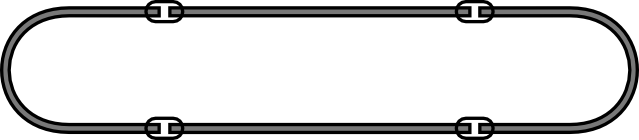
\includegraphics[width=0.6\textwidth]{png/tasma}
  \caption{Taśma przenośnikowa w uproszczeniu}
  \label{fig:belt-drw}
\end{figure}

Element Belt jest jedynie elementem grupującym i nie ma swojej fizycznej
reprezentacji w konstrukcji przenośnika taśmowego. Element ten definiuje
strukturę, zgodnie z którą taśma przenośnikowa jest listą naprzemiennie
występujących elementów BeltSegment oraz BeltSplice, gdzie położenie tych
elementów w dokumencie odzwierciedla położenie odcinków i złącz w rzeczywistej
taśmie zamontowanej na przenośniku. Pierwsze złącze na liście łączy ze sobą
odcinek następujący bezpośrednio po nim oraz ostatni odcinek na liście, w ten
sposób domykając pętlę.

\begin{verbatim}
<Belt>
  <BeltSplice id="1" />
  <BeltSegment id="2" />
  <BeltSplice id="3" />
  <BeltSegment id="4" />
  <BeltSplice id="5" />
  <BeltSegment id="6" />
</Belt>
\end{verbatim}

W powyższym listingu odcinek taśmy 6 jest połączony złączem 5 z odcinkiem taśmy
4 oraz złączem 1 z odcinkiem taśmy 2. W najprostszym przypadku może być jedno
złącze i jeden odcinek.

\begin{figure}[h]
  \centering
  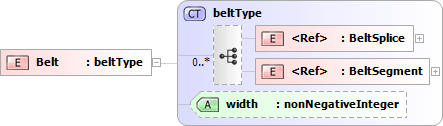
\includegraphics[width=0.6\textwidth]{png/belt_xsd2}
  \caption{Definicja elementu Belt}
  \label{fig:belt-xsd}
\end{figure}

\paragraph{Definicje atrybutów:}
\begin{description}
\item[width] Szerokość taśmy - B [mm].
\end{description}


\subsubsection{Odcinek taśmy <BeltSegment>}
Element BeltSegment odzwierciedla fizycznie zamontowany na przenośniku odcinek
taśmy.  Atrybuty z grupy \emph{beltSegmentAttrGroup} mogą występować
bezpośrednio w elemencie BeltSegment lub elemencie BeltSegmentType do którego
można się odwoływać z elementu Belt segment za pomocą atrybutu
\emph{type}. Cechą tej grupy atrybutów jest to, że mogą opisywać zarówno
instancję jak i typ odcinka taśmy. Atrybuty length oraz cetificate mogą
występować tylko w elemencie BeltSegment.

\begin{figure}[h]
  \centering
  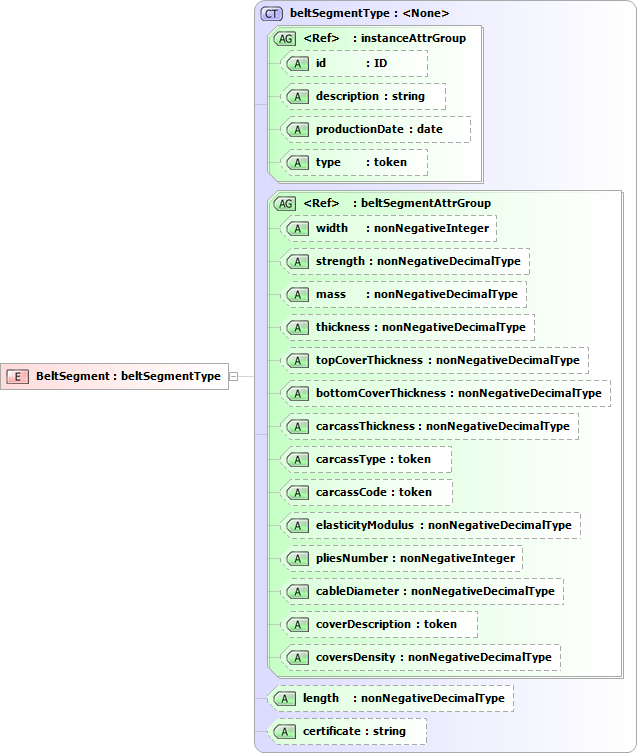
\includegraphics[width=0.6\textwidth]{png/belt_segment_xsd2}
  \caption{Definicja elementu BeltSegment}
  \label{fig:beltSegment-xsd}
\end{figure}

\paragraph{Definicje atrybutów:}
\begin{description}
\item[width] Szerokość odcinka taśmy [mm]
\item[strength] Nominalna wytrzymałość taśmy [kN/m]
\item[mass] Masa taśmy [kg/m]
\item[thickness] Grubość taśmy [mm]
\item[topCoverThickness] Grubość okładki górnej (nośnej) [mm]
\item[bottomCoverThickness] Grubość okładki dolnej (bieżnej) [mm]
\item[carcassThickness] Grubość rdzenia taśmy [mm]
\item[carcassType] Typ rdzenia taśmy (tkaninowa, z linkami stalowymi)
\item[carcassCode] Współczynnik rodzaju materiału rdzenia
\item[elasticityModulus] Moduł sprężystości taśmy - E [kN/m]
\item[pliesNumber] Liczba przekładek lub linek
\item[cableDiameter] Średnica linki [mm]
\item[coverDescription] Oznaczenie okładek
\item[coversDensity] Gęstość mieszanki okładkowej [kg/mm*m$^2$]
\item[length] Długość odcinka [m]
\item[certificate] Numer atestu
\end{description}


\subsubsection{Złącze <BeltSplice>}
Złącze w języku ConvML odnosi się do sąsiednich elementów na liście potomków
elementu Belt. W poprawnym dokumencie będą to zawsze elementy BeltSegment
reprezentujące odcinki taśmy. Złącze w przeciwieństwie do odcinka nie posiada
parametru długości i jest rozpatrywane jako miejsce (punkt) wykonania
połączenia.

\begin{figure}[h]
  \centering
  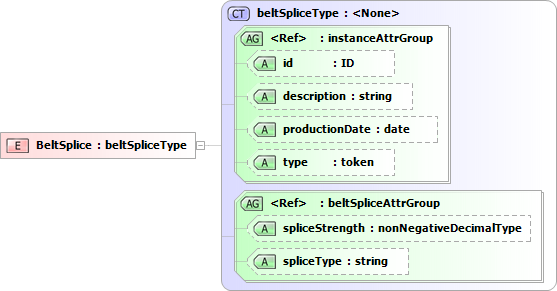
\includegraphics[width=0.6\textwidth]{png/belt_splice_xsd2}
  \caption{Definicja elementu BeltSplice}
  \label{fig:beltSplice-xsd}
\end{figure}

W przypadku złącza, standardowy atrybut \emph{productionDate} należy tłumaczyć
jako datę wykonania złącza.

\paragraph{Definicje atrybutów:}
\begin{description}
\item[spliceStrength] Wytrzymałość połączenia [\%]
\item[spliceType] Rodzaj złącza np: wulkanizowane, mechaniczne, klejone, inne.
\end{description}


\subsection{Stacja zwrotna <Tail>}
Stacja zwrotna jest elementem konstrukcyjnym przenośnika taśmowego w którym taśma
zmienia kierunek ruchu z trasy dolnej (powrotnej) na trasę górną (nosną). Zmiana
kierunku odbywa się na bębnie zwrotnym, który jest pierwszym podelementem elementu
Tail w strukturze. Elementy Carry oraz Return odpowiadają trasie niśnej oraz trasie
powrotnej i są opisane w rozdziale dotyczącym segmentów trasy.

\begin{figure}[h]
  \centering
  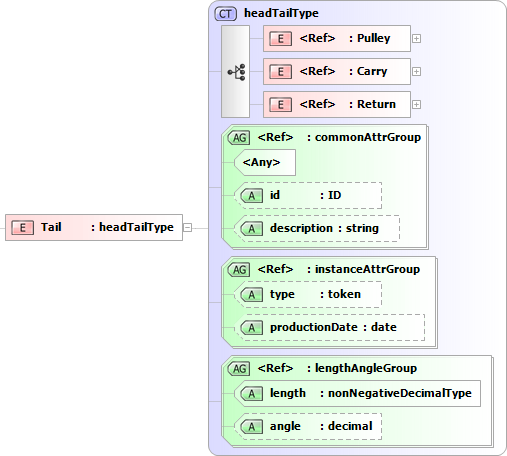
\includegraphics[width=0.6\textwidth]{png/liquid/Tail}
  \caption{Definicja elementu Tail}
  \label{fig:tail-xsd}
\end{figure}


\subsection{Stacja czołowa <Head>}
Stacja czołowa pomimo innej nazwy elementu w stosuku do stacji zwrotnej posiada dokładnie
taką samą definicję podemenetów. Zmienia sie jedynie interpretacja elementu Pulley, który
w tym przypdaku odpowiada bebnowi czołowemu i obywa się na nim zmiana kierunku taśmy z
trasy nośnej na trasę powrotną.

\begin{figure}[h]
  \centering
  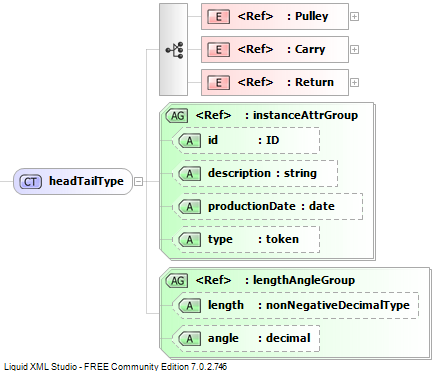
\includegraphics[width=0.6\textwidth]{png/liquid/headTailType}
  \caption{Definicja typu elementu Head}
  \label{fig:headTailType-xsd}
\end{figure}


\subsection{Bęben <Pulley>}
Element Pulley reprezentuje bęben w strukturze przenośnika. Poza bębenami zwrotnym oraz
czołowym, które posiadają określone miejsca w strukturze, można umieścić dodatkowe bębny
w strukturze przenośnika jako podelementy elementów Carry (górna trasa) oraz Return (dolna
trasa).

Ze względu na funkcję rozróżnia się w przenosnikach bębny napędowe; napinające,
zapewniające niezbędne napięcie taśmy; odchylające lub odginające, zwększające kąt
opasania taśmy.

W języku ConvML bębny wszystkich rodzajów oznacza się tym samym elementem
Pulley. O ich funkcji decydują elementy zawarte wewnątrz elementu Pulley. Przy braku
tych elementów bęben pełni funkcję odchylającą. Przy obecności jednego lub dwóch
zestawów napędowych (DriveUnit) staje się bębnem napędowym. Analogicznie obecność
zestawu napinającego (TakeUpSystem) informuje o funkcji napinającej bębna, 

\begin{figure}[h]
  \centering
  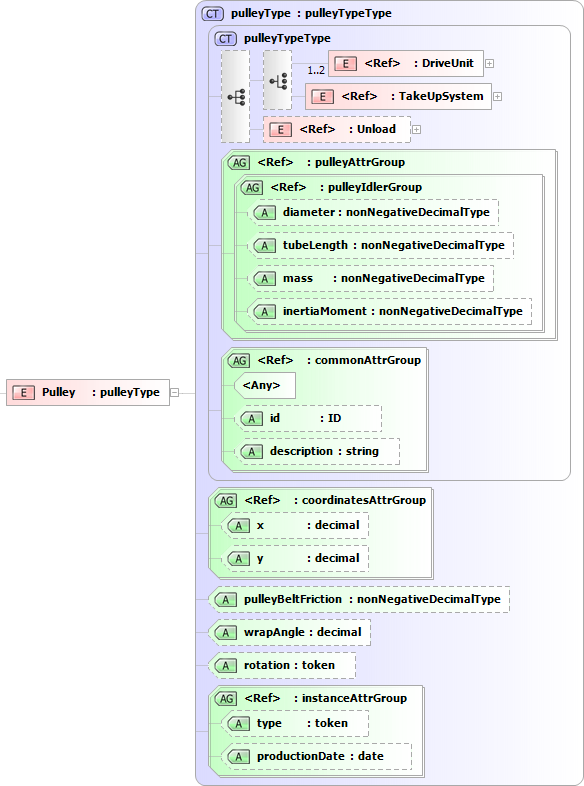
\includegraphics[width=0.6\textwidth]{png/liquid/Pulley}
  \caption{Definicja elementu Pulley}
  \label{fig:pulley-xsd}
\end{figure}


\subsection{Trasa <Route>}


\subsubsection{Odcinek trasy <RouteSection>}
Odcinek trasy jest elementem logicznego podziału trasy przenośnika na elementy o róznej
długości oraz nachyleniu. Podział na odcinki umożliwia zapis podstawowych parametrów
geometrycznych przenośnika.

Do najważniejszych atrybutów elementu RouteSection należą length oraz angle. 


\subsubsection{Segment trasy <RouteSegment>}
Segement trasy jest fizycznym elementem konstrukcyjnym który umożliwa montaż podzespołów
współpracyjących z taśmą poruszającą się na trasie powrotnej lub nośnej. 

\subsubsection{Górna trasa <Carry>}


\subsubsection{Dolna trasa <Return>}


\subsection{Zespół napędowy <DriveUnit>}

\begin{figure}[h]
  \centering
  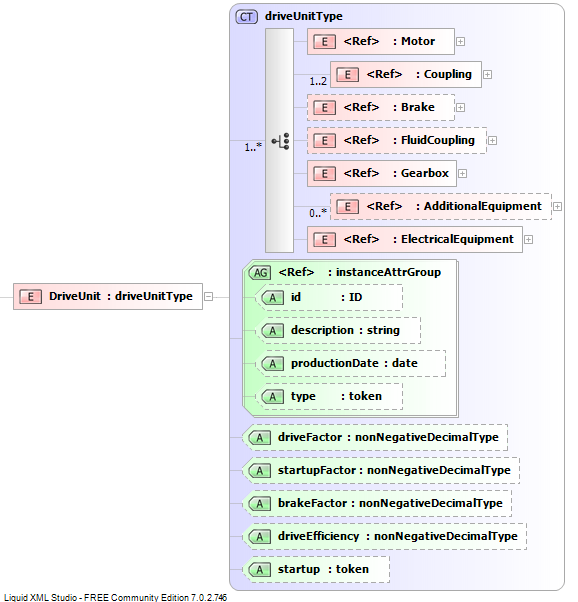
\includegraphics[width=0.6\textwidth]{png/liquid/DriveUnit}
  \caption{Definicja elementu DriveUnit}
  \label{fig:driveUnit-xsd}
\end{figure}


\subsubsection{Silnik <Motor>}

\begin{figure}[h]
  \centering
  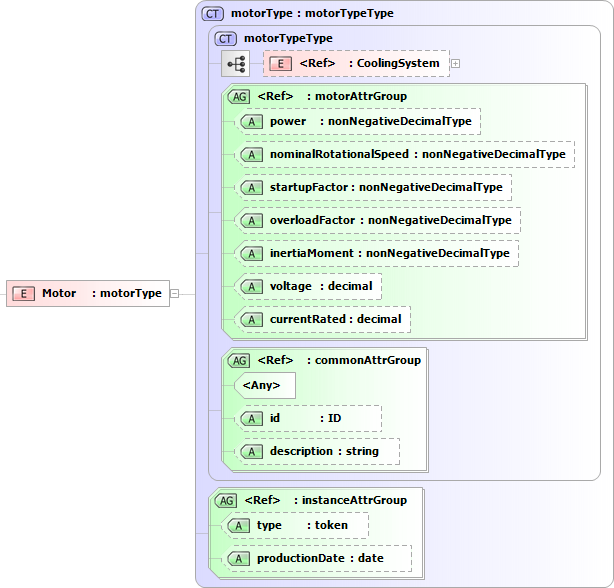
\includegraphics[width=0.6\textwidth]{png/liquid/Motor}
  \caption{Definicja elementu Motor}
  \label{fig:motor-xsd}
\end{figure}


\subsubsection{Sprzęgło podatne <Coupling>}

\begin{figure}[h]
  \centering
  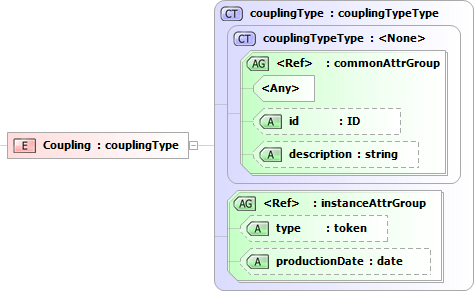
\includegraphics[width=0.6\textwidth]{png/liquid/Coupling}
  \caption{Definicja elementu Coupling}
  \label{fig:coupling-xsd}
\end{figure}


\subsubsection{Sprzęgło hydrodynamiczne <FluidCoupling>}

\begin{figure}[h]
  \centering
  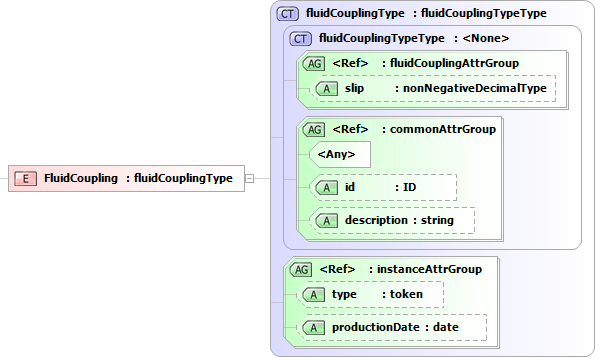
\includegraphics[width=0.6\textwidth]{png/liquid/FluidCoupling}
  \caption{Definicja elementu FluidCoupling}
  \label{fig:fluidCoupling-xsd}
\end{figure}


\subsubsection{Układ hamulcowy <Break>}

\begin{figure}[h]
  \centering
  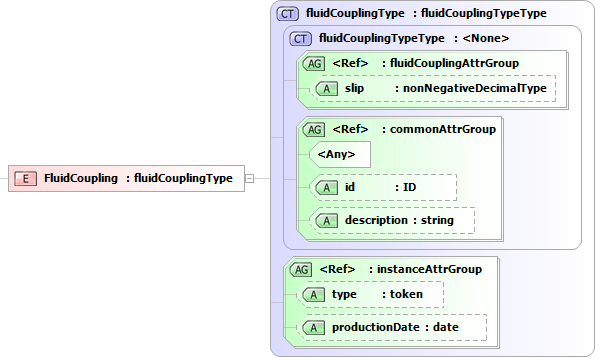
\includegraphics[width=0.6\textwidth]{png/liquid/FluidCoupling}
  \caption{Definicja elementu Break}
  \label{fig:break-xsd}
\end{figure}


\subsubsection{Przekładnia <Gearbox>}

\begin{figure}[h]
  \centering
  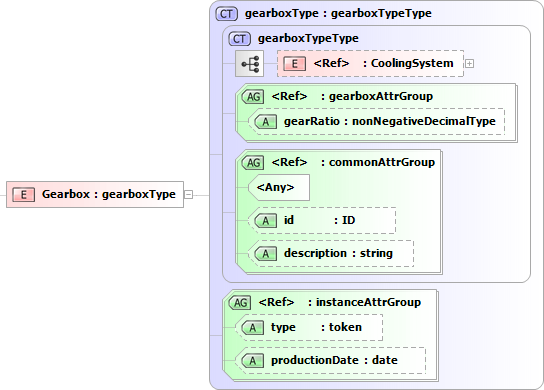
\includegraphics[width=0.6\textwidth]{png/liquid/Gearbox}
  \caption{Definicja elementu Gearbox}
  \label{fig:gearbox-xsd}
\end{figure}


\subsection{Zespół napinający <TakeUpSystem>}

\begin{figure}[h]
  \centering
  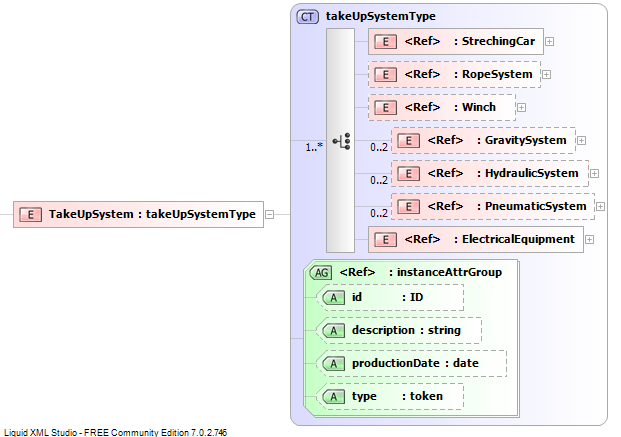
\includegraphics[width=0.6\textwidth]{png/liquid/TakeUpSystem}
  \caption{Definicja elementu TakeUpSystem}
  \label{fig:takeUpSystem-xsd}
\end{figure}


\subsubsection{Wózek napinający <StrechingCar>}

\begin{figure}[h]
  \centering
  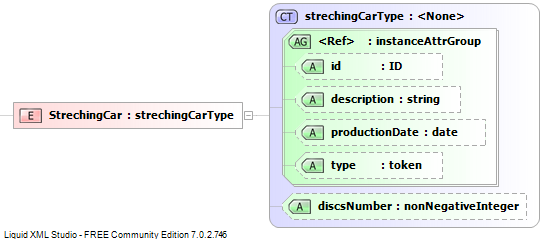
\includegraphics[width=0.6\textwidth]{png/liquid/StrechingCar}
  \caption{Definicja elementu StrechingCar}
  \label{fig:strechingCar-xsd}
\end{figure}


\subsubsection{Układ zlinowania <RopeSystem>}

\begin{figure}[h]
  \centering
  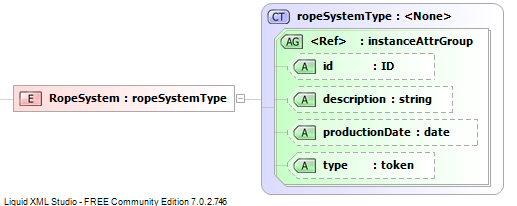
\includegraphics[width=0.6\textwidth]{png/liquid/RopeSystem}
  \caption{Definicja elementu RopeSystem}
  \label{fig:ropeSystem-xsd}
\end{figure}


\subsubsection{Wciagarka <Winch>}


\subsubsection{Układ grawitacyjny <GravitySystem>}


\subsubsection{Układ hydrauliczny <HydraulicSystem>}


\subsubsection{Układ pneumatyczny <PneumaticSystem>}


\subsection{Rozładunek <Unload>}


\subsection{Elementy trasy}


\subsection{Wyposażenie elektryczne przenosnika <ConvElectricalEquipment>}


\subsubsection{Układ sterowania przenośnikiem <ControlSystem>}


\subsubsection{System wyłączenia awaryjnego <EmergencySystem>}


\subsubsection{System łączności i sygnalizacji <SignalSystem>}


\subsubsection{Instalacja przeciwpożarowa <FireSystem>}


\subsection{Pozostałe}
tutaj opisać: Urządzenie dodatkowe, Wyposażenie elektryczne urządzenia, Układ chłodzenia


\section{Typy <Types>}

Do formatu ConvML w wersji 1.2 wprowadzono pojęcie typu w celu uniknięca niepotrzebnych
powtórzeń.  Typ w sensie rozumianym przez ConvML jest zbiorem wartości atrubutów, które
mogą być współdzielone przez wiele instancji tego samego elementu.
Typy definiuje się wewnątrz elementu Types, a ich nazwa tworzona jest poprzez dodanie
do nazwy elementu sufiksu Type. Każdy Typ musi posiadać unikalny atrybut typeId.

Instancja elementu BeltSegment dziedziczy wartości atrybutów zdefinowanych w elemencie
BeltSegmentType jeśli wartość atrybutu type zgadza się z wartościa atrybutu typeId.

UWAGA! Czy powinno być dopuszczalne przedefiniowywanie atrybutów?

\begin{verbatim}
<Types>
  <BeltSegmentType typeId="GTP-1200/t"
                   bottomCoverThickness="2"
                   carcassType="tekstylny"
                   coverDescription="trudnopalna"
                   elasticityModulus="2000"
                   manufacturer="Wolbrom"
                   pliesNumber="3"
                   topCoverThickness="4"
                   width="1200"/>
</Types>
\end{verbatim}

\begin{verbatim}
<Belt>
  <BeltSplice/>
  <BeltSegment type="GTP-1200/t"
               length="100"
               productionDate="2005-04-11"
               certificate="1257"/>
  <BeltSplice/>
  <BeltSegment type="GTP-1200/t"
               length="100"
               productionDate="2005-07-15"
               certificate="1258"/>
</Belt>
\end{verbatim}

\end{document}
